% generated from JIRA project LVV
% using template at /Users/krughoff/lsst_stack/conda/miniconda3-py38_4.9.2/envs/docsteady-env/lib/python3.7/site-packages/docsteady/templates/tpr.latex.jinja2.
% using docsteady version 2.2.3
% Please do not edit -- update information in Jira instead
\documentclass[dm,STR,toc]{lsstdoc}
\usepackage{geometry}
\usepackage{longtable,booktabs}
\usepackage{enumitem}
\usepackage{arydshln}
\usepackage{attachfile}
\usepackage{array}
\usepackage{dashrule}

\newcolumntype{L}[1]{>{\raggedright\let\newline\\\arraybackslash\hspace{0pt}}p{#1}}

\input meta.tex

\newcommand{\attachmentsUrl}{https://github.com/\gitorg/\lsstDocType-\lsstDocNum/blob/\gitref/attachments}
\providecommand{\tightlist}{
  \setlength{\itemsep}{0pt}\setlength{\parskip}{0pt}}

\setcounter{tocdepth}{4}

\begin{document}

\def\milestoneName{EFD on Summit for M1/M3}
\def\milestoneId{DM-503-EFDa}
\def\product{Data Management}

\setDocCompact{true}

\title{DM-503-EFDa: EFD on Summit for M1/M3 Test Plan and Report}
\setDocRef{\lsstDocType-\lsstDocNum}
\date{ 2021-09-21 }
\author{ Simon Krughoff }

% Most recent last
\setDocChangeRecord{
\addtohist{}{2021-03-23}{First draft}{K. Simon Krughoff}
\addtohist{}{2021-09-21}{Draft for review}{K. Simon Krughoff}
}

\setDocCurator{K. Simon Krughoff}
\setDocUpstreamLocation{\url{https://github.com/lsst-dm/\lsstDocType-\lsstDocNum}}
\setDocUpstreamVersion{\vcsRevision}



\setDocAbstract{
This is the test plan and report for
\textbf{ EFD on Summit for M1/M3} (DM-503-EFDa),
an LSST milestone pertaining to the Data Management Subsystem.\\
This document is based on content automatically extracted from the Jira test database on \docDate.
The most recent change to the document repository was on \vcsDate.
}


\maketitle

\section{Introduction}
\label{sect:intro}


\subsection{Objectives}
\label{sect:objectives}

 The purpose of this test plan is to describe all the necessary
requirements and infrastructure for successfully testing the Engineering
Facility Database (EFD) as implemented with Kafka, InfluxDB and
Chronograf. This plan will describe the prerequisites for beginning a
test campaign, step by step instructions for each test can and a
description of the expected results and test
artifacts.\\[2\baselineskip]NB: The use of the term reliability in this
document is intended to indicate the number of messages produced
relative to the number of messages recorded in the EFD. The system shall
be considered reliable if at least 99.9\% of produced messages are
recorded.\\[2\baselineskip]The highest level description of this test
plan is to run the M1/M3 subsystem in an active state for no less than 5
contiguous days. During this time, all telemetry produced by the M1/M3
subsystem will appear in the InfluxDB instance running at the summit
with latency less than 4 seconds 99\% of the time. The maximum latency
shall be less than 20 seconds. All telemetry shall also be available for
interrogation by Chronograf on similar time scales. Any gap in telemetry
or dropped/missing messages will be considered a deviation. Successful
completion of the test campaign will show that:\\

\begin{enumerate}
\tightlist
\item
  ~users are able to access data ingested in the InfluxDB at the summit
  in near real time from the Chronograf interface
\item
  the latency from message production to ingestion in InfluxDB is less
  than the nominal limit (4 sec) 99\% of the time and never more than 20
  seconds during nominal operation
\item
  the M1/M3 telemetry is successfully being mirrored to another influxDB
  instance at the data facility with latency less than 24 hours under
  normal circumstances (e.g. no network outages). ~Though the
  requirement flowed down from project and data management subsystem
  requirement documents is 24 hours, this exercise will quantify the
  realized latency. ~We expect the typical latency to be less than 20
  seconds. With the maximum latency being less than 5 minutes.
\item
  users are able to access and analyze telemetry data from the M1/M3
  subsystem from notebooks running in the notebook aspect of the RSP
  both at the summit and at the data facility\\
\end{enumerate}



\subsection{System Overview}
\label{sect:systemoverview}

 The tests will be carried out from within an instance of the notebook
aspect of the RSP running at either the summit or the data facility. An
appropriate weekly version of the stack will be chosen.


\subsection{Document Overview}
\label{sect:docoverview}

This document was generated from Jira, obtaining the relevant information from the
\href{https://jira.lsstcorp.org/secure/Tests.jspa\#/testPlan/LVV-P78}{LVV-P78}
~Jira Test Plan and related Test Cycles (
\href{https://jira.lsstcorp.org/secure/Tests.jspa\#/testCycle/LVV-C163}{LVV-C163}
).

Section \ref{sect:intro} provides an overview of the test campaign, the system under test (\product{}),
the applicable documentation, and explains how this document is organized.
Section \ref{sect:testplan} provides additional information about the test plan, like for example the configuration
used for this test or related documentation.
Section \ref{sect:personnel} describes the necessary roles and lists the individuals assigned to them.

Section \ref{sect:overview} provides a summary of the test results, including an overview in Table \ref{table:summary},
an overall assessment statement and suggestions for possible improvements.
Section \ref{sect:detailedtestresults} provides detailed results for each step in each test case.

The current status of test plan \href{https://jira.lsstcorp.org/secure/Tests.jspa\#/testPlan/LVV-P78}{LVV-P78} in Jira is \textbf{ Approved }.

\subsection{References}
\label{sect:references}
\renewcommand{\refname}{}
\bibliography{lsst,refs,books,refs_ads,local}


\newpage
\section{Test Plan Details}
\label{sect:testplan}


\subsection{Data Collection}

  Observing is not required for this test campaign.

\subsection{Verification Environment}
\label{sect:hwconf}
  The environment will be largely within notebooks running a modern stack,
though for the first test case and interactive environment is necessary.
~In that case commands will be executed with a notebook. ~The results of
those commands will be viewed in the summit version of the chronograf
interface.

  \subsection{Entry Criteria}
  \begin{enumerate}
\tightlist
\item
  Before beginning this test, as set of viability tests shall be
  performed. These will show:

  \begin{enumerate}
  \tightlist
  \item
    The system demonstrates reliability (number of recorded
    messages/number of produced messages) of greater than 99.9\%
  \item
    The typical latency of the system is less than 4 sec for a pre
    defined set of topics
  \item
    The summit data is being replicated to the instance at NCSA
  \item
    Chronograf is set up and running at both the summit and NCSA
  \end{enumerate}
\item
  The summit network and Kubernetes cluster are performing nominally
\item
  The EFD is deployed in the summit Kubernetes cluster
\item
  The M1M3 sub-component is reliably producing telemetry via Kafka
  producers with correct versions of the schema
\item
  The notebook aspect of the RSP is deployed in the summit Kubernetes
  cluster
\item
  The summit EFD is reliably replicated to an EFD instance running in a
  data facility
\item
  The notebook aspect of the RSP is deployed in the same data facility
  as that running the replicated EFD
\item
  The most recent version of the EFD client python modules are installed
  in the various deployed notebook aspects
\item
  A requirement test that the system demonstrates reliability of greater
  than 99.9\%
\end{enumerate}



\subsection{Related Documentation}


\begin{longtable}{rp{10cm}l}
\multicolumn{3}{c}{Jira Attachments} \\ \hline
 To LVV-C163 results &
  LVV-T2111-report.pdf & \attachfile{attachments/LVV-T2111-report.pdf}\\ \hline
To LVV-C163 results &
  Slew\_with\_M1M3.ipynb & \attachfile{attachments/Slew_with_M1M3.ipynb}\\ \hline
To LVV-C163 results &
  mt\_utils.py & \attachfile{attachments/mt_utils.py}\\ \hline
 To LVV-C163 results &
  LVV-T2112.ipynb & \attachfile{attachments/LVV-T2112.ipynb}\\ \hline
To LVV-C163 results &
  summit\_M1M3\_forceActuatorData.log & \attachfile{attachments/summit_M1M3_forceActuatorData.log}\\ \hline
To LVV-C163 results &
  summit\_M1M3\_heartbeat.log & \attachfile{attachments/summit_M1M3_heartbeat.log}\\ \hline
To LVV-C163 results &
  summit\_M1M3\_forceActuatorData(1).py & \attachfile{attachments/summit_M1M3_forceActuatorData(1).py}\\ \hline
To LVV-C163 results &
  summit\_M1M3\_heartbeat(1).py & \attachfile{attachments/summit_M1M3_heartbeat(1).py}\\ \hline
 To LVV-C163 results &
  summit\_M1M3\_heartbeat(2).py & \attachfile{attachments/summit_M1M3_heartbeat(2).py}\\ \hline
To LVV-C163 results &
  LVV-T2117.ipynb & \attachfile{attachments/LVV-T2117.ipynb}\\ \hline
To LVV-C163 results &
  sept\_hbeat.log & \attachfile{attachments/sept_hbeat.log}\\ \hline
 To LVV-C163 results &
  LVV-T2116.ipynb & \attachfile{attachments/LVV-T2116.ipynb}\\ \hline
 To LVV-C163 results &
  LVV-T2115(1).ipynb & \attachfile{attachments/LVV-T2115(1).ipynb}\\ \hline
   \end{longtable}

All documents provided as attachments in Jira are downloaded to Github and linked here for convenience.
However, since they are not properly versioned, they should be considered informal and therefore
not be part of the verification baseline.


\subsection{PMCS Activity}

Primavera milestones related to the test campaign:
\begin{itemize}
\item DM-503-EFDa
\end{itemize}


\newpage
\section{Personnel}
\label{sect:personnel}

The personnel involved in the test campaign is shown in the following table.

{\small
\begin{longtable}{p{3cm}p{3cm}p{3cm}p{6cm}}
\hline
\multicolumn{2}{r}{T. Plan \href{https://jira.lsstcorp.org/secure/Tests.jspa\#/testPlan/LVV-P78}{LVV-P78} owner:} &
\multicolumn{2}{l}{\textbf{ Simon Krughoff } }\\\hline
\multicolumn{2}{r}{T. Cycle \href{https://jira.lsstcorp.org/secure/Tests.jspa\#/testCycle/LVV-C163}{LVV-C163} owner:} &
\multicolumn{2}{l}{\textbf{
Simon Krughoff }
} \\\hline
\textbf{Test Cases} & \textbf{Assigned to} & \textbf{Executed by} & \textbf{Additional Test Personnel} \\ \hline
\href{https://jira.lsstcorp.org/secure/Tests.jspa#/testCase/LVV-T2111}{LVV-T2111}
& {\small Simon Krughoff } & {\small Simon Krughoff } &
\begin{minipage}[]{6cm}
\smallskip
{\small  }
\medskip
\end{minipage}
\\ \hline
\href{https://jira.lsstcorp.org/secure/Tests.jspa#/testCase/LVV-T2112}{LVV-T2112}
& {\small Simon Krughoff } & {\small Simon Krughoff } &
\begin{minipage}[]{6cm}
\smallskip
{\small  }
\medskip
\end{minipage}
\\ \hline
\href{https://jira.lsstcorp.org/secure/Tests.jspa#/testCase/LVV-T2117}{LVV-T2117}
& {\small Simon Krughoff } & {\small Simon Krughoff } &
\begin{minipage}[]{6cm}
\smallskip
{\small  }
\medskip
\end{minipage}
\\ \hline
\href{https://jira.lsstcorp.org/secure/Tests.jspa#/testCase/LVV-T2116}{LVV-T2116}
& {\small Simon Krughoff } & {\small Simon Krughoff } &
\begin{minipage}[]{6cm}
\smallskip
{\small  }
\medskip
\end{minipage}
\\ \hline
\href{https://jira.lsstcorp.org/secure/Tests.jspa#/testCase/LVV-T2115}{LVV-T2115}
& {\small Simon Krughoff } & {\small Simon Krughoff } &
\begin{minipage}[]{6cm}
\smallskip
{\small  }
\medskip
\end{minipage}
\\ \hline
\end{longtable}
}

\newpage

\section{Test Campaign Overview}
\label{sect:overview}

\subsection{Summary}
\label{sect:summarytable}

{\small
\begin{longtable}{p{2cm}cp{2.3cm}p{8.6cm}p{2.3cm}}
\toprule
\multicolumn{2}{r}{ T. Plan \href{https://jira.lsstcorp.org/secure/Tests.jspa\#/testPlan/LVV-P78}{LVV-P78}:} &
\multicolumn{2}{p{10.9cm}}{\textbf{ DM-503-EFDa: EFD on Summit for M1/M3 }} & Approved \\\hline
\multicolumn{2}{r}{ T. Cycle \href{https://jira.lsstcorp.org/secure/Tests.jspa\#/testCycle/LVV-C163}{LVV-C163}:} &
\multicolumn{2}{p{10.9cm}}{\textbf{ DM-503-EFDa: EFD on Summit for M1/M3 }} & Done \\\hline
\textbf{Test Cases} &  \textbf{Ver.} & \textbf{Status} & \textbf{Comment} & \textbf{Issues} \\\toprule
\href{https://jira.lsstcorp.org/secure/Tests.jspa#/testCase/LVV-T2111}{LVV-T2111}
&  2
& Pass &
\begin{minipage}[]{9cm}
\smallskip

\medskip
\end{minipage}
&   \\\hline
\href{https://jira.lsstcorp.org/secure/Tests.jspa#/testCase/LVV-T2112}{LVV-T2112}
&  1
& Pass &
\begin{minipage}[]{9cm}
\smallskip

\medskip
\end{minipage}
&   \\\hline
\href{https://jira.lsstcorp.org/secure/Tests.jspa#/testCase/LVV-T2117}{LVV-T2117}
&  1
& Pass &
\begin{minipage}[]{9cm}
\smallskip

\medskip
\end{minipage}
&   \\\hline
\href{https://jira.lsstcorp.org/secure/Tests.jspa#/testCase/LVV-T2116}{LVV-T2116}
&  1
& Pass &
\begin{minipage}[]{9cm}
\smallskip

\medskip
\end{minipage}
&   \\\hline
\href{https://jira.lsstcorp.org/secure/Tests.jspa#/testCase/LVV-T2115}{LVV-T2115}
&  1
& Pass &
\begin{minipage}[]{9cm}
\smallskip

\medskip
\end{minipage}
&   \\\hline
\caption{Test Campaign Summary}
\label{table:summary}
\end{longtable}
}

\subsection{Overall Assessment}
\label{sect:overallassessment}

Not yet available.

\subsection{Recommended Improvements}
\label{sect:recommendations}

Not yet available.

\newpage
\section{Detailed Test Results}
\label{sect:detailedtestresults}

\subsection{Test Cycle LVV-C163 }

Open test cycle {\it \href{https://jira.lsstcorp.org/secure/Tests.jspa#/testrun/LVV-C163}{DM-503-EFDa: EFD on Summit for M1/M3}} in Jira.

Test Cycle name: DM-503-EFDa: EFD on Summit for M1/M3\\
Status: Done



\subsubsection{Software Version/Baseline}
Not provided.

\subsubsection{Configuration}
Not provided.

\subsubsection{Test Cases in LVV-C163 Test Cycle}

\paragraph{ LVV-T2111 - Access to M1/M3 telemetry data in near real time via the Chronograf
interface }\mbox{}\\

Version \textbf{2}.
Open  \href{https://jira.lsstcorp.org/secure/Tests.jspa#/testCase/LVV-T2111}{\textit{ LVV-T2111 } }
test case in Jira.

Show that users can get access to visualizations in Chronograf with
telemetry arriving in less than 5 seconds from a command run on the DDS
network.

\textbf{ Preconditions}:\\
See prerequisites in the Test Plan LVV-P78

Execution status: {\bf Pass }

Final comment:\\


Detailed steps results:

\begin{tabular}{p{2cm}p{14cm}}
\toprule
Step 1 & Step Execution Status: \textbf{ Pass } \\ \hline
\end{tabular}
 Description \\
{\footnotesize
Log in to whatever VPNs are necessary to both see Chronograf at the NCSA
test stand (NTS) and the control network necessary for commanding
components fo the M1/M3 subsystem

}
\hdashrule[0.5ex]{\textwidth}{1pt}{3mm}
  Expected Result \\
{\footnotesize
VPN connects are live

}
\hdashrule[0.5ex]{\textwidth}{1pt}{3mm}
  Actual Result \\
{\footnotesize
In the attached video VPN login begins at 00:00 and finishes at 00:45.
~The Cisco VPN client is configured to attach to the VPN server at NCSA.
~After entering my Kerberos password and ``push'' as the second
password, a 2FA challenge arrived on my phone which was answered. ~Note
that the login process took longer than it normally does. ~This is
attributed to load on the computer since it was simultaneously doing the
screen recording.

}
\begin{tabular}{p{2cm}p{14cm}}
\toprule
Step 2 & Step Execution Status: \textbf{ Pass } \\ \hline
\end{tabular}
 Description \\
{\footnotesize
Log in to chronograf running at the NTS. The endpoint is currently
\href{https://lsst-chronograf-nts-efd.ncsa.illinois.edu/}{https://lsst-chronograf-nts-efd.ncsa.illinois.edu},
though \href{https://sqr-034.lsst.io/}{https://sqr-034.lsst.io} shall be
considered the primary source of truth for service endpoints relating to
the EFD

}
\hdashrule[0.5ex]{\textwidth}{1pt}{3mm}
  Expected Result \\
{\footnotesize
The browser showing the front page of the chronograf interface

}
\hdashrule[0.5ex]{\textwidth}{1pt}{3mm}
  Actual Result \\
{\footnotesize
At 01:10 in the attached video I navigate to the Chronograf URL, namely
https://lsst-chronograf-nts-efd.ncsa.illinois.edu/. ~Login is via github
authentication. ~In this case, my access token was already cached by my
browser. ~If it had not been, there would been a login cycle through the
GitHub authentication flow.

}
\begin{tabular}{p{2cm}p{14cm}}
\toprule
Step 3 & Step Execution Status: \textbf{ Pass } \\ \hline
\end{tabular}
 Description \\
{\footnotesize
Open the dashboard labeled ``Test Case 1 LVV-P78''

}
\hdashrule[0.5ex]{\textwidth}{1pt}{3mm}
  Expected Result \\
{\footnotesize
There should be several panes all showing a different trace for the time
window of now() - 1hr

}
\hdashrule[0.5ex]{\textwidth}{1pt}{3mm}
  Actual Result \\
{\footnotesize
At 01:25 I have navigated to to the dashboard created for this test
case: ``Test Case 1 LVV-P78''. ~The six panels show up. ~Some have data
in them and some of them do not because the time window is the past 15
minutes. ~Chronograf remembers the time window you last specified, so we
did not get the 1hr default. ~I do not believe this is a deviation since
the intent was simply to show the dashboard in the default state which
is what was done on my system.

}
\begin{tabular}{p{2cm}p{14cm}}
\toprule
Step 4 & Step Execution Status: \textbf{ Pass } \\ \hline
\end{tabular}
 Description \\
{\footnotesize
Set the refresh in chronograph to 5 seconds and adjust the time window
to show the past 15 minutes of data. Both of these operations are done
using buttons immediately above the graph window on the right side

}
\hdashrule[0.5ex]{\textwidth}{1pt}{3mm}
  Expected Result \\
{\footnotesize
\begin{itemize}
\tightlist
\item
  The trace is now the last 15 minutes and the view refreshes every 5
  seconds
\item
  The query used to produce the trace plots will be captured as an
  artifact
\end{itemize}

}
\hdashrule[0.5ex]{\textwidth}{1pt}{3mm}
  Actual Result \\
{\footnotesize
These settings are applied at 01:25 - 01:50 in the attached video. ~In
consultation with Michael Reuter, we decided to make the time window 5
minutes instead of 15 minutes since the test only lasts about 5 minutes.
~This allows us to see more detail in the traces as they scroll by.~ The
suggested refresh rate of 5 seconds was preserved.

}
\begin{tabular}{p{2cm}p{14cm}}
\toprule
Step 5 & Step Execution Status: \textbf{ Pass } \\ \hline
\end{tabular}
 Description \\
{\footnotesize
Issue a series of commands to the M1M3 subsystem via a notebook.

}
\hdashrule[0.5ex]{\textwidth}{1pt}{3mm}
  Expected Result \\
{\footnotesize
\begin{itemize}
\tightlist
\item
  Confirmation that the command was acted upon
\item
  This will also include a qualitative description of whether the
  command produced the expected change in telemetry.
\item
  The notebook executing the commands will be captured as an artifact
\end{itemize}

}
\hdashrule[0.5ex]{\textwidth}{1pt}{3mm}
  Actual Result \\
{\footnotesize
At 01:50 control was handed over to Michael to execute the commands in
his notebook. ~Through the duration of the test, several commands are
issued. ~See the attached notebook for the exact commands. ~The
telemetry observed in Chronograf tracked with the expected values. ~The
one oddity is that the ``Hardpoint Corrections'' command reports
``false'' when they are turned on. ~This is a convention used with some
CSCs where the value in the command is not important, just that the
command was issued.\\[2\baselineskip]Note that there are some
convenience functions used in the notebook that are defined in the
included helper library.

}
\begin{tabular}{p{2cm}p{14cm}}
\toprule
Step 6 & Step Execution Status: \textbf{ Pass } \\ \hline
\end{tabular}
 Description \\
{\footnotesize
Verify new values are showing up in the summit instance of InfluxDB by
observing that values with newer timestamps are appearing in the
Chronograf visualization

}
\hdashrule[0.5ex]{\textwidth}{1pt}{3mm}
  Expected Result \\
{\footnotesize
Record the session using a screen capture tool

}
\hdashrule[0.5ex]{\textwidth}{1pt}{3mm}
  Actual Result \\
{\footnotesize
From 01:50 to 07:25 Michael continues to execute the notebook.
~Throughout, the telemetry tracks with what is being commanded by the
notebook. ~We can see the traces update almost immediately modulo the 5
second refresh rate throughout. ~There was no noticeable lag at all.

}
\begin{tabular}{p{2cm}p{14cm}}
\toprule
Step 7 & Step Execution Status: \textbf{ Pass } \\ \hline
\end{tabular}
 Description \\
{\footnotesize
Produce a report for the test

}
\hdashrule[0.5ex]{\textwidth}{1pt}{3mm}
  Expected Result \\
{\footnotesize
\begin{itemize}
\tightlist
\item
  A document explaining the procedure including the topics monitored,
  the command issued and the query used to do the visualization
\end{itemize}

}
\hdashrule[0.5ex]{\textwidth}{1pt}{3mm}
  Actual Result \\
{\footnotesize
The document has been attached to the test case. ~Note that the video
was too large to attach to the final report because of GitHub hosting
limits. ~A link to the video is available
\href{https://lsst.ncsa.illinois.edu/~krughoff/data/TC1-LVV-P78-take2-trimmed.mp4}{here}.

}

\paragraph{ LVV-T2112 - Latency from production to ingestion and telemetry can be analyzed via
notebooks: High and Low Cadence }\mbox{}\\

Version \textbf{1}.
Open  \href{https://jira.lsstcorp.org/secure/Tests.jspa#/testCase/LVV-T2112}{\textit{ LVV-T2112 } }
test case in Jira.

Measure the latency of production to ingestion in the EFD and show it is
less than 4 seconds 99\% of the time.\\
Show that this analysis can be completed via a notebook running in an
instance of the notebook aspect of the RSP.

\textbf{ Preconditions}:\\
See prerequisites in the Test Plan LVV-P78

Execution status: {\bf Pass }

Final comment:\\


Detailed steps results:

\begin{tabular}{p{2cm}p{14cm}}
\toprule
Step 1 & Step Execution Status: \textbf{ Pass } \\ \hline
\end{tabular}
 Description \\
{\footnotesize
Log in to whatever VPNs are necessary to access to the summit notebook
aspect of the RSP

}
\hdashrule[0.5ex]{\textwidth}{1pt}{3mm}
  Expected Result \\
{\footnotesize
VPN connection is active

}
\hdashrule[0.5ex]{\textwidth}{1pt}{3mm}
  Actual Result \\
{\footnotesize
I am logged into the summit VPN via the tunnelblick client using my IPA
account credentials.

}
\begin{tabular}{p{2cm}p{14cm}}
\toprule
Step 2 & Step Execution Status: \textbf{ Pass } \\ \hline
\end{tabular}
 Description \\
{\footnotesize
Log in to the summit notebook aspect: https://summit-lsp.lsst.codes/nb\\
Make sure to choose a recent weekly and a large instance

}
\hdashrule[0.5ex]{\textwidth}{1pt}{3mm}
  Expected Result \\
{\footnotesize
The JupyterLab interface is displayed in the browser

}
\hdashrule[0.5ex]{\textwidth}{1pt}{3mm}
  Actual Result \\
{\footnotesize
I have logged into the summit instance of the nublado service using the
above URL. ~I am using the following image with a large container:
Weekly 2021\_37 (SAL Cycle 0021, Build 005)

}
\begin{tabular}{p{2cm}p{14cm}}
\toprule
Step 3 & Step Execution Status: \textbf{ Pass } \\ \hline
\end{tabular}
 Description \\
{\footnotesize
Open a notebook:

\begin{enumerate}
\tightlist
\item
  Navigate to the File-\textgreater{}New-\textgreater{}Notebook
\item
  When prompted, select the LSST kernel
\end{enumerate}

}
\hdashrule[0.5ex]{\textwidth}{1pt}{3mm}
  Expected Result \\
{\footnotesize
An empty notebook running in the LSST kernel

}
\hdashrule[0.5ex]{\textwidth}{1pt}{3mm}
  Actual Result \\
{\footnotesize
I have open in the JupyterLab interface a notebook running the LSST
kernel as indicated in the upper right and in the ``Idle'' state as
indicated in the bottom status bar.

}
\begin{tabular}{p{2cm}p{14cm}}
\toprule
Step 4 & Step Execution Status: \textbf{ Pass } \\ \hline
\end{tabular}
 Description \\
{\footnotesize
Connect to the summit EFD

}
\hdashrule[0.5ex]{\textwidth}{1pt}{3mm}
  Example Code \\
{\footnotesize
from lsst\_efd\_client import EfdClient\\
efd = EfdClient('summit\_efd')

}
\hdashrule[0.5ex]{\textwidth}{1pt}{3mm}
  Expected Result \\
{\footnotesize
A notebook with an instance of the `EfdClient` configured to talk to the
summit EFD

}
\hdashrule[0.5ex]{\textwidth}{1pt}{3mm}
  Actual Result \\
{\footnotesize
It turns out we couldn't do this study via a direct query of the EFD
because of technical reasons I will explain in a later step, but we do
still need to use the EFD to query for periods of time where the MTM1M3
subsystem was down for one reason or another. ~Thus, it is still
important for us to set up a connection to the summit EFD at this
point.\\[2\baselineskip]I now have, in my notebook, an instance of the
EfdClient class connected to the ``summit\_efd'' instance.

}
\begin{tabular}{p{2cm}p{14cm}}
\toprule
Step 5 & Step Execution Status: \textbf{ Pass } \\ \hline
\end{tabular}
 Description \\
{\footnotesize
Choose a topic to query and select a 5 day window of data. The topic and
window are arbitrary, but it shall be explicit (not relative to now())
so that it can reproduced. The topic shall be one of high enough cadence
that there are many measurements for the topic, i.e. not a command or
log topic that could potentially be very sparsely populated over the 5
day window. A high cadence, ideally greater than 20 Hz, topic will give
the most precise measurement of the distribution of the latency.

}
\hdashrule[0.5ex]{\textwidth}{1pt}{3mm}
  Expected Result \\
{\footnotesize
\begin{itemize}
\tightlist
\item
  A table-like object in memory containing data from the chosen topic
  and time window.
\item
  The window and topic are artifacts to be preserved
\end{itemize}

}
\hdashrule[0.5ex]{\textwidth}{1pt}{3mm}
  Actual Result \\
{\footnotesize
We chose the `lsst.sal.MTM1M3.forceActuatorData' topic since it is
sampled at 50 Hz natively. ~It is also a particularly wide topic, so
represents one of the topics with the most throughput in the MTM1M3
subsystem. ~The time window chose is 2021-05-24T21:43:31.853 to
2021-05-29T21:43:31.853 in TAI. ~This odd chose for time window is
explained in the following step.\\[2\baselineskip]I now have a numpy
array with the various timestamps necessary to compute the latency in
memory in my notebook.

}
\begin{tabular}{p{2cm}p{14cm}}
\toprule
Step 6 & Step Execution Status: \textbf{ Pass } \\ \hline
\end{tabular}
 Description \\
{\footnotesize
\begin{enumerate}
\tightlist
\item
  The total latency is the time from the message being published,
  private\_sndStamp, and when it is ingested in the influxDB database.
  Currently the index timestamp is private\_sndStamp There will be an
  additional field added to the measurement to reflect the ingest
  timestamp. This may be technically difficult, in which case a subset
  of topics will have an extra column added by hand for the purpose of
  this analysis. Care shall also be taken to ensure the messages are in
  the same (TAI) time system. In the past some CSCs have been reporting
  TAI and some report UTC. Currently, the difference is 37 seconds.
\item
  Compute the total latency by taking the difference of the two columns,
  arr{[}`timestamp'{]} - arr{[}`private\_sndStamp'{]} (this is where
  correction for TAI/UTC would be included if necessary). The result
  shall be in seconds.
\end{enumerate}

}
\hdashrule[0.5ex]{\textwidth}{1pt}{3mm}
  Expected Result \\
{\footnotesize
An array-like object in memory containing the latency in seconds for
every message in the window

}
\hdashrule[0.5ex]{\textwidth}{1pt}{3mm}
  Actual Result \\
{\footnotesize
It turned out that it was too hard to add an actual field containing the
ingestion time of each message. ~This has to do with the way data is
transferred from kafka to influxdb. ~Instead, we chose an alternative
approach where we used the EFD client to poll particular topics looking
for the last ingested message. ~For very high frequency data, this is a
proxy for the ingest time for that message. ~For lower frequency topics,
the resolution of measured latency is limited by the topic
frequency.\\[2\baselineskip]We ran the process querying the EFD for the
most recent messages for the duration of the nominal operating window of
5 days and then beyond. The timestamps from the messages are logged into
a file on disk along with the machine time immediately before doing the
query and immediately after the query. This log file is then imported
into the notebook to provide the data used to compute the latencies
presented here.\\[2\baselineskip]In addition to the log data, it's
necessary to account for gaps in the telemetry for two reasons:

\begin{enumerate}
\tightlist
\item
  There were several times faults occurred. ~We simply mask over those
  time windows by inspecting the EFD for the appropriate states. ~Any
  time the state changes to something other than ENABLED, we mark the
  beginning of a gap in the telemetry. ~When the state changes back to
  ENABLED, we mark the end of that gap.
\item
  On two occasions services went down without the normal warning in the
  state. ~Once it was a hard crash of the MTM1M3 system that prevented
  changing into a non-ENABLED state before it went off line. ~The other
  was when my polling script was killed because of maintenance on
  nublado at the summit. ~Both of these gaps in the data were recorded
  and are applied in the same way the EFD defined gaps are
\end{enumerate}

There is one more filtering step that is necessary. In some instances,
the query arrives in influxDB before a message has been completely
ingested. This results in the log file containing NaN values for the
missing information. I have spot checked and confirmed that the data in
influxDB is consistent, but these data are not useful for computing
latencies. This is a rare occurrence and does not impact the statistics
of the analysis.\\[2\baselineskip]We took the beginning of the analysis
window to simply be the first message in the log file produced by the
polling script.\\[2\baselineskip]I now have two arrays in memory. Once
containing the time for every message and one containing the latency for
every message in seconds.\\[2\baselineskip]See the attached script,
summit\_M1M3\_forceActuatorData.py, for the exact script run to record
these data.

}
\begin{tabular}{p{2cm}p{14cm}}
\toprule
Step 7 & Step Execution Status: \textbf{ Pass } \\ \hline
\end{tabular}
 Description \\
{\footnotesize
Count the number of entries less than 4 seconds and divide that by the
total number of entries. This value shall be greater than or equal to
99\%.

}
\hdashrule[0.5ex]{\textwidth}{1pt}{3mm}
  Expected Result \\
{\footnotesize
\begin{itemize}
\tightlist
\item
  A plot showing a histogram of the latency values indicating the 99\%
  value.
\item
  If the 99\% latency is greater than 4 sec, an explanation shall be
  supplied describing why the latency is higher than expected more often
  than expected
\item
  The plot shall also indicate the maximum latency observed
\item
  If the maximum latency is above the nominal maximum (20 sec), an
  explanation shall be provided
\end{itemize}

}
\hdashrule[0.5ex]{\textwidth}{1pt}{3mm}
  Actual Result \\
{\footnotesize
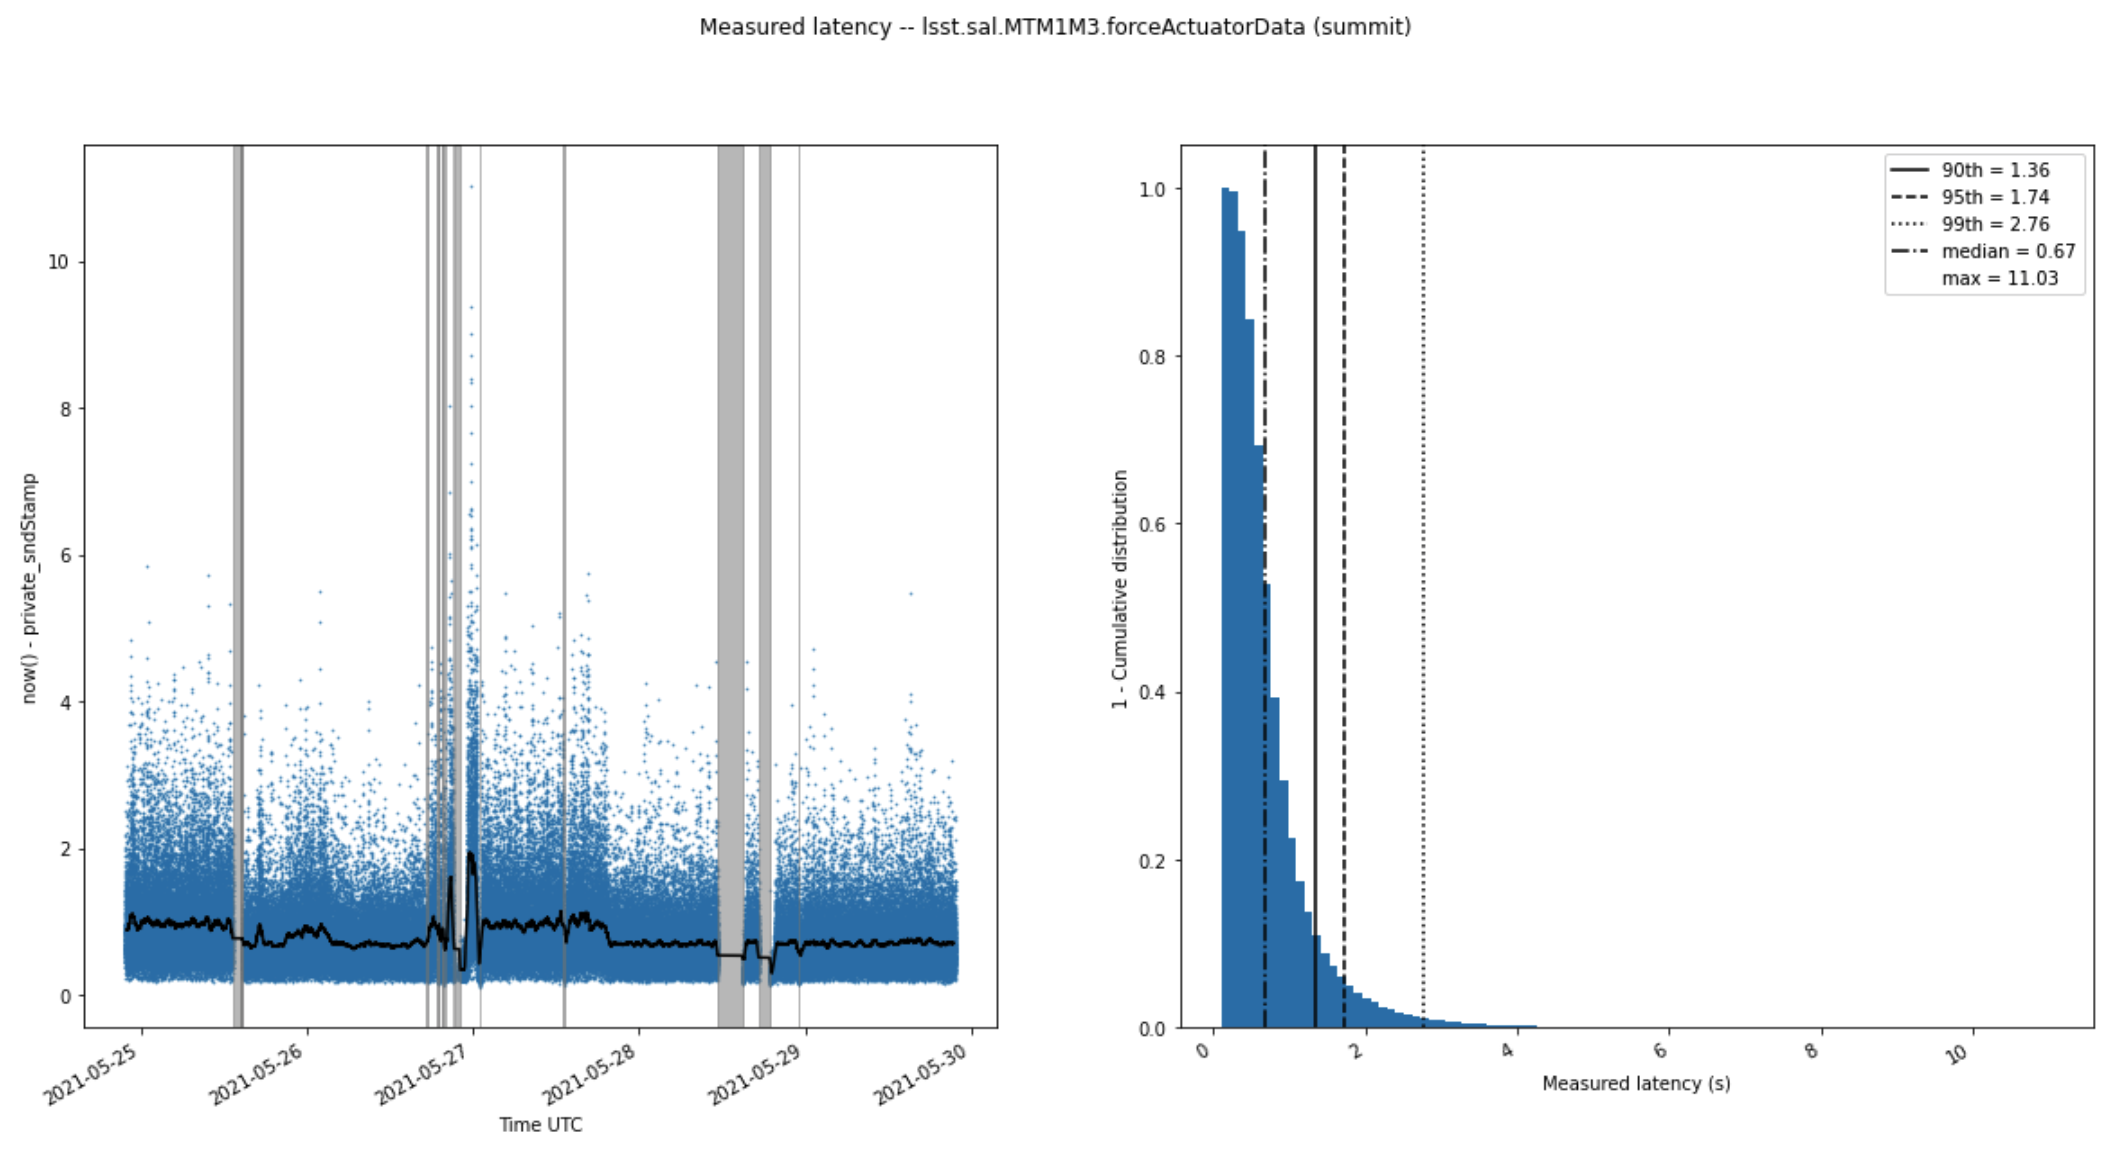
\includegraphics[width=3.73958in]{jira_imgs/1842.png}The attached plot
shows the distribution of latency as a function of time over the 5 days
on the left and shows the distribution of latency values on the right.
The bars are the gaps. Data from those regions was excluded. The median,
90th percentile, 95th percentile, and 99th percentile are plotted in the
right pane as vertical lines. This shows that we meet the less than 4
seconds 99\% of the time. 4 seconds represents the 99.8th percentile for
this dataset which is greater than the 99\% required by this test.
Maximum latency is 11.03 seconds.\\[2\baselineskip]These values all meet
the expected results, so additional explanation is necessary.

}
\begin{tabular}{p{2cm}p{14cm}}
\toprule
Step 8 & Step Execution Status: \textbf{ Pass } \\ \hline
\end{tabular}
 Description \\
{\footnotesize
Choose a topic to query and select a 5 day window of data. The topic and
window are arbitrary, but it shall be explicit (not relative to now())
so that it can reproduced. The topic shall be low latency in order to to
measure the impact of publishing low and high latency topics
simultaneously

}
\hdashrule[0.5ex]{\textwidth}{1pt}{3mm}
  Expected Result \\
{\footnotesize
\begin{itemize}
\tightlist
\item
  A table-like object in memory containing data from the chosen topic
  and time window.
\item
  The window and topic are artifacts to be preserved
\end{itemize}

}
\hdashrule[0.5ex]{\textwidth}{1pt}{3mm}
  Actual Result \\
{\footnotesize
For the low latency topic, we choose the
``lsst.sal.MTM1M3.logevent\_heartbeat'' which is an aliveness topic that
publishes a message with minimal content every second. ~We choose the
same time window as for the high frequency topic:
2021-05-24T21:43:31.853 to 2021-05-29T21:43:31.853 in
TAI.\\[2\baselineskip]I have read the logging file into memory and have
a numpy array with the timestamps.

}
\begin{tabular}{p{2cm}p{14cm}}
\toprule
Step 9 & Step Execution Status: \textbf{ Pass } \\ \hline
\end{tabular}
 Description \\
{\footnotesize
\begin{enumerate}
\tightlist
\item
  The total latency is the time from the message being published,
  private\_sndStamp, and when it is ingested in the influxDB database.
  Currently the index timestamp is private\_sndStamp There will be an
  additional field added to the measurement to reflect the ingest
  timestamp. This may be technically difficult, in which case a subset
  of topics will have an extra column added by hand for the purpose of
  this analysis. Care shall also be taken to ensure the messages are in
  the same (TAI) time system. In the past some CSCs have been reporting
  TAI and some report UTC. Currently, the difference is 37 seconds.
\item
  Compute the total latency by taking the difference of the two columns,
  arr{[}`timestamp'{]} - arr{[}`private\_sndStamp'{]} (this is where
  correction for TAI/UTC would be included if necessary). The result
  shall be in seconds.
\end{enumerate}

}
\hdashrule[0.5ex]{\textwidth}{1pt}{3mm}
  Expected Result \\
{\footnotesize
An array-like object in memory containing the latency in seconds for
every message in the window

}
\hdashrule[0.5ex]{\textwidth}{1pt}{3mm}
  Actual Result \\
{\footnotesize
We follow the same process as step 6 for filtering and producing the
latency values. ~Note that because the latency of the topic is 1 second
and the polling happens every second, the uncertainly in the measured
latency can be up to a second.\\[2\baselineskip]See the attached script,
summit\_M1M3\_heartbeat.py, for the exact script run to record these
data.

}
\begin{tabular}{p{2cm}p{14cm}}
\toprule
Step 10 & Step Execution Status: \textbf{ Pass } \\ \hline
\end{tabular}
 Description \\
{\footnotesize
Count the number of entries less than 4 seconds and divide that by the
total number of entries. This value shall be greater than or equal to
99\%. ~This is intended to show that even when publishing simultaneously
with high and low cadence topics we still meet the latency goal for both
topics

}
\hdashrule[0.5ex]{\textwidth}{1pt}{3mm}
  Expected Result \\
{\footnotesize
\begin{itemize}
\tightlist
\item
  A plot showing a histogram of the latency values indicating the 99\%
  value.
\item
  If the 99\% latency is greater than 4 sec, an explanation shall be
  supplied describing why the latency is higher than expected more often
  than expected
\item
  The plot shall also indicate the maximum latency observed
\item
  If the maximum latency is above the nominal maximum (20 sec), an
  explanation shall be provided
\end{itemize}

}
\hdashrule[0.5ex]{\textwidth}{1pt}{3mm}
  Actual Result \\
{\footnotesize
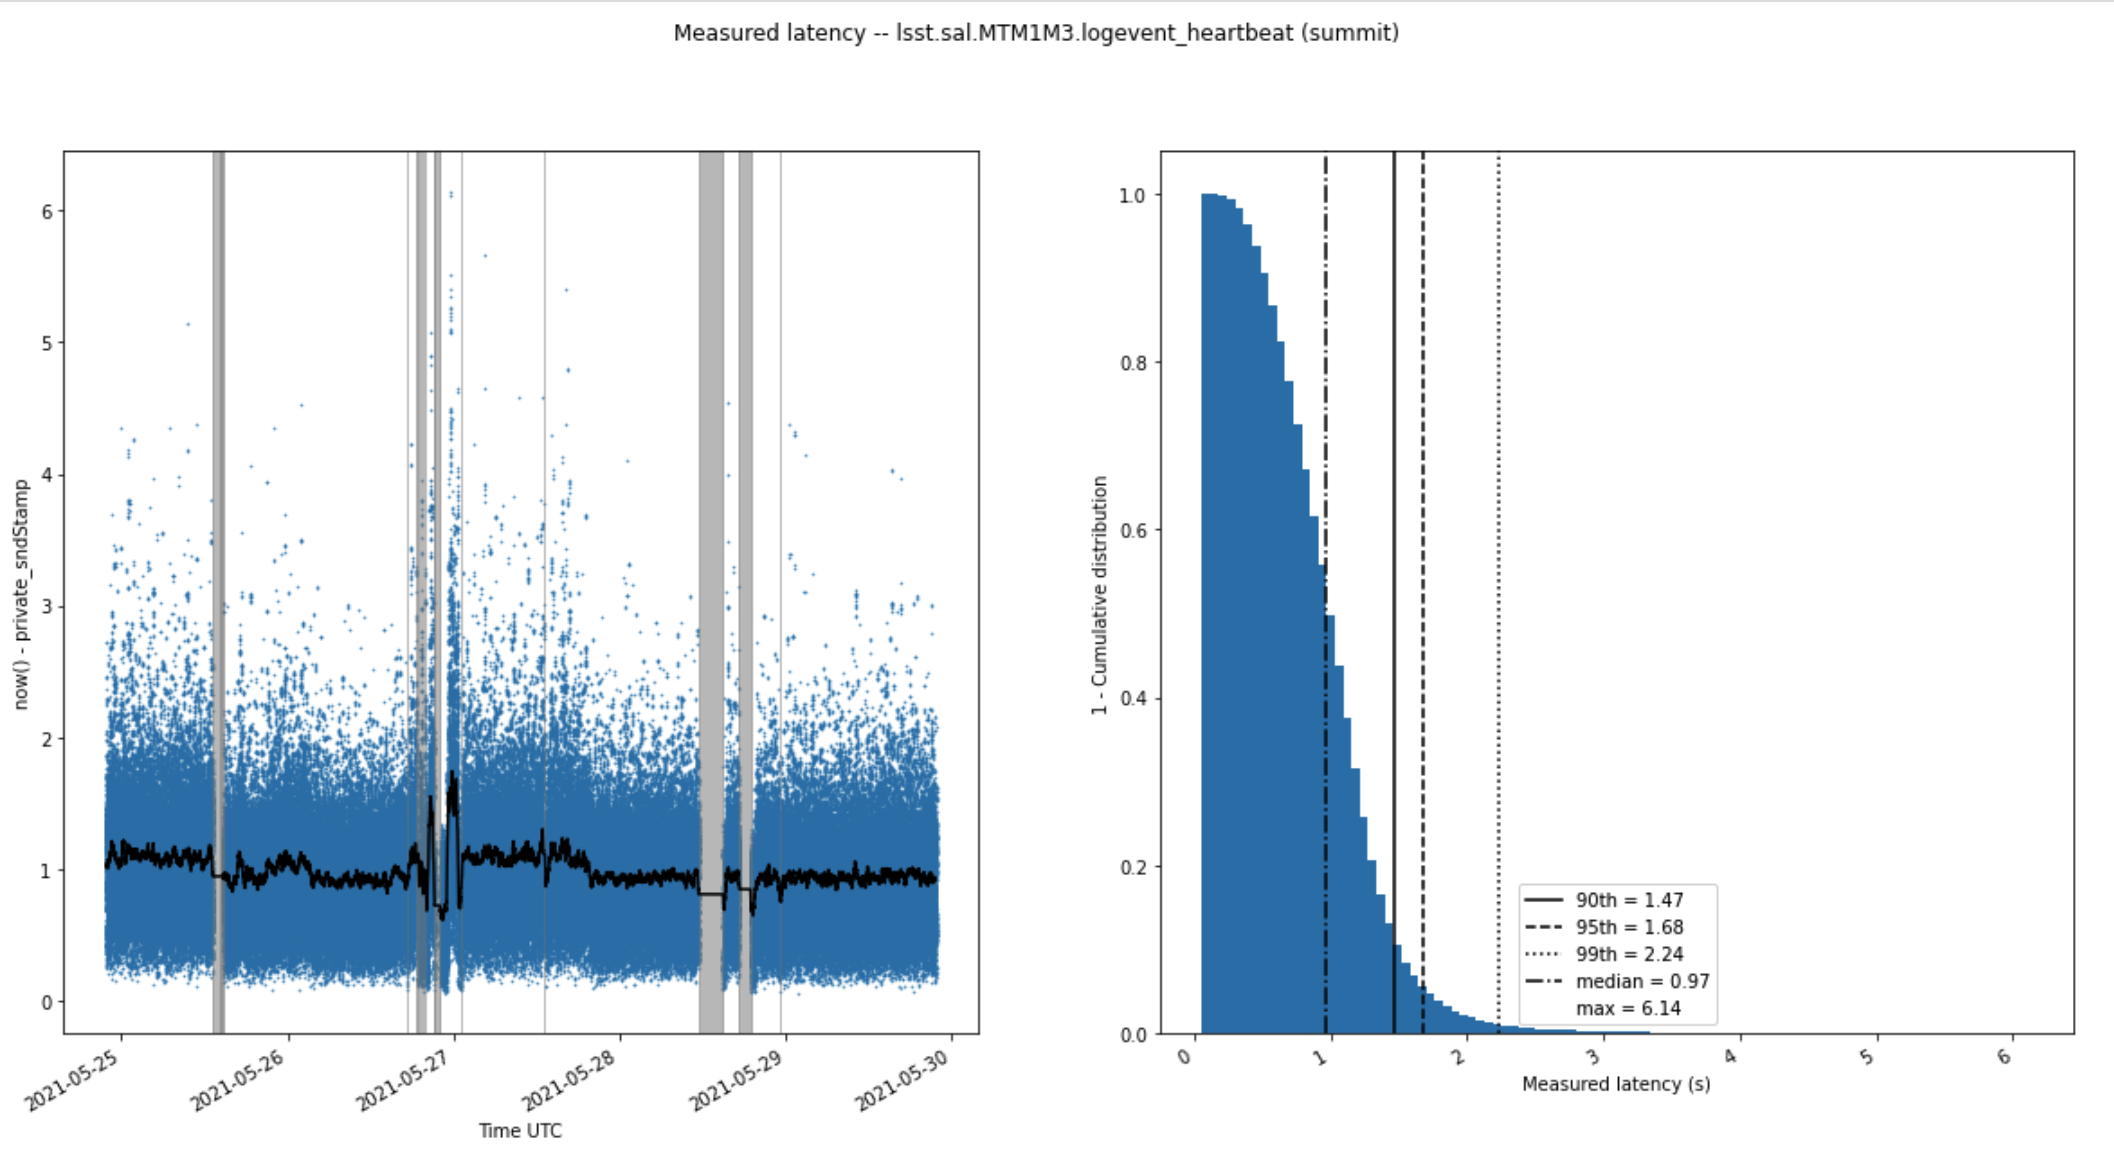
\includegraphics[width=3.37500in]{jira_imgs/1844.png}As expected, the
median of the distribution is around 1 second. ~This is because of the
uncertainty in the measurement of the latency. ~Taking this into
account, the scatter for the low frequency topic is significantly
smaller than the high frequency topic. ~It also easily fits in the 4
second envelope. 4 seconds is the 99.98th percentile for this
distribution. ~The maximum latency over this window is 6.14 seconds.

}
\begin{tabular}{p{2cm}p{14cm}}
\toprule
Step 11 & Step Execution Status: \textbf{ Pass } \\ \hline
\end{tabular}
 Description \\
{\footnotesize
Document the procedure including latency distributions, time window, and
both high and low cadence topics

}
\hdashrule[0.5ex]{\textwidth}{1pt}{3mm}
  Expected Result \\
{\footnotesize
\begin{itemize}
\tightlist
\item
  A document describing the process including the topic chosen and the
  time window.
\item
  The document shall be in the form on a notebook with saved outputs, or
  an instance of an nbreport.
\end{itemize}

}
\hdashrule[0.5ex]{\textwidth}{1pt}{3mm}
  Actual Result \\
{\footnotesize
See the attached notebook. ~The associated data files are also necessary
to run the notebook to completion.\\[2\baselineskip]The scripts used to
do the logging are also included as attachments to this test script.

}

\paragraph{ LVV-T2117 - Latency from production to ingestion and telemetry can be analyzed via
notebooks: Low Cadence }\mbox{}\\

Version \textbf{1}.
Open  \href{https://jira.lsstcorp.org/secure/Tests.jspa#/testCase/LVV-T2117}{\textit{ LVV-T2117 } }
test case in Jira.

Measure the latency of production to ingestion in the EFD and show it is
less than 4 seconds 99\% of the time.\\
Show that this analysis can be completed via a notebook running in an
instance of the notebook aspect of the RSP.

\textbf{ Preconditions}:\\
See prerequisites in the Test Plan LVV-P78

Execution status: {\bf Pass }

Final comment:\\


Detailed steps results:

\begin{tabular}{p{2cm}p{14cm}}
\toprule
Step 1 & Step Execution Status: \textbf{ Pass } \\ \hline
\end{tabular}
 Description \\
{\footnotesize
Log in to whatever VPNs are necessary to access to the summit notebook
aspect of the RSP

}
\hdashrule[0.5ex]{\textwidth}{1pt}{3mm}
  Expected Result \\
{\footnotesize
VPN connection is active

}
\hdashrule[0.5ex]{\textwidth}{1pt}{3mm}
  Actual Result \\
{\footnotesize
I am logged into the summit EFD via the tunnelblick client with my IPA
credentials.

}
\begin{tabular}{p{2cm}p{14cm}}
\toprule
Step 2 & Step Execution Status: \textbf{ Pass } \\ \hline
\end{tabular}
 Description \\
{\footnotesize
Log in to the summit notebook aspect: https://summit-lsp.lsst.codes/nb\\
Make sure to choose a recent weekly and a large instance

}
\hdashrule[0.5ex]{\textwidth}{1pt}{3mm}
  Expected Result \\
{\footnotesize
The JupyterLab interface is displayed in the browser

}
\hdashrule[0.5ex]{\textwidth}{1pt}{3mm}
  Actual Result \\
{\footnotesize
I am logged into the notebook aspect of the RSP via the URL:
https://summit-lsp.lsst.codes/nb. ~I have chosen a large container
running the following image version: Weekly 2021\_37 (SAL Cycle 0021,
Build 005). ~I now see the JupyterLab interface in my browser.

}
\begin{tabular}{p{2cm}p{14cm}}
\toprule
Step 3 & Step Execution Status: \textbf{ Pass } \\ \hline
\end{tabular}
 Description \\
{\footnotesize
Open a notebook:

\begin{enumerate}
\tightlist
\item
  Navigate to the File-\textgreater{}New-\textgreater{}Notebook
\item
  When prompted, select the LSST kernel
\end{enumerate}

}
\hdashrule[0.5ex]{\textwidth}{1pt}{3mm}
  Expected Result \\
{\footnotesize
An empty notebook running in the LSST kernel

}
\hdashrule[0.5ex]{\textwidth}{1pt}{3mm}
  Actual Result \\
{\footnotesize
I have an open empty notebook running the LSST kernel as indicated in
the upper right of the notebook. ~It is currently in the Idle state
according to the status indicator in the bottom bar of the JupyterLab
interface.

}
\begin{tabular}{p{2cm}p{14cm}}
\toprule
Step 4 & Step Execution Status: \textbf{ Pass } \\ \hline
\end{tabular}
 Description \\
{\footnotesize
Connect to the summit EFD

}
\hdashrule[0.5ex]{\textwidth}{1pt}{3mm}
  Example Code \\
{\footnotesize
from lsst\_efd\_client import EfdClient\\
efd = EfdClient('summit\_efd')

}
\hdashrule[0.5ex]{\textwidth}{1pt}{3mm}
  Expected Result \\
{\footnotesize
A notebook with an instance of the `EfdClient` configured to talk to the
summit EFD

}
\hdashrule[0.5ex]{\textwidth}{1pt}{3mm}
  Actual Result \\
{\footnotesize
As discussed in the next cell, the assumption when this test case was
written was that we would query the EFD directly for the latency, but
for technical reasons, this was not possible. ~An in situ measurement of
the latency was necessary. ~In other test cases, the EFD client was used
to figure out when the system was running by querying the system state,
but in this case we specifically wish to observe the system when the
M1M3 sub-system may be in states other than
``ENABLED''.\\[2\baselineskip]For these reasons, we do not actually need
a connection to an active EFD to successfully complete the rest of this
test case. ~For completeness. ~We show that it was possible to create
the client, even if it's not strictly needed.

}
\begin{tabular}{p{2cm}p{14cm}}
\toprule
Step 5 & Step Execution Status: \textbf{ Pass } \\ \hline
\end{tabular}
 Description \\
{\footnotesize
Choose a topic to query and select a 5 day window of data. The topic and
window are somewhat arbitrary, but it shall be explicit (not relative to
now()) so that it can reproduced. The topic shall be a low cadence topic
with reasonably even sampling. ~I.e. not a command or event topic that
could be very sparse and unevenly sampled. ~The window should be chosen
specifically to be during a period where high cadence topics are not
publishing at peak, so as to measure the latency of the low cadence
topics on a quiescent network.

}
\hdashrule[0.5ex]{\textwidth}{1pt}{3mm}
  Expected Result \\
{\footnotesize
\begin{itemize}
\tightlist
\item
  A table-like object in memory containing data from the chosen topic
  and time window.
\item
  The window and topic are artifacts to be preserved
\end{itemize}

}
\hdashrule[0.5ex]{\textwidth}{1pt}{3mm}
  Actual Result \\
{\footnotesize
I chose a window over the last 5 days: 2021-09-15T20:24:09.054 --
2021-09-20T20:24:09.054. ~ The start time was simply the time of the
first message I logged, and then the window was set for 5 days following
that. ~I was under the impression that the M1M3 sub-system would be
fairly quiet now. ~It turns out that there was some work that happened
during my window. ~This was verified by
\href{https://lsstc.slack.com/archives/C01P41NUR1R/p1631798190100500}{slack
comments} in the \#summit-announce channel. There wasn't a specific time
listed in the slack message, but inspecting the EFD indicates that they
started around 09:00 local and finished around 19:30 local. I therefore
put a filter over that time to prevent the statistics from being
influenced over a period where the system was in active use and therefor
not quiescent. That time window is: 2021-09-16T12:00Z --
2021-09-16T20:45Z.\\[2\baselineskip]The topic chosen is the same one
used in the high latency tests: ``lsst.sal.MTM1M3.logevent\_heartbeat''.
The difference here is that we are trying to see how the low frequency
topics behave when the high frequency topics are not being driven at
their maximum load.\\[2\baselineskip]After loading the log file produced
by the latency measurement script described in the next step, the
notebook now has a table with timestamps from the local machine time and
the timestamps reported in the messages for the measurements in the
window.

}
\begin{tabular}{p{2cm}p{14cm}}
\toprule
Step 6 & Step Execution Status: \textbf{ Pass } \\ \hline
\end{tabular}
 Description \\
{\footnotesize
\begin{enumerate}
\tightlist
\item
  The total latency is the time from the message being published,
  private\_sndStamp, and when it is ingested in the influxDB database.
  Currently the index timestamp is private\_sndStamp There will be an
  additional field added to the measurement to reflect the ingest
  timestamp. This may be technically difficult, in which case a subset
  of topics will have an extra column added by hand for the purpose of
  this analysis. Care shall also be taken to ensure the messages are in
  the same (TAI) time system. In the past some CSCs have been reporting
  TAI and some report UTC. Currently, the difference is 37 seconds.
\item
  Compute the total latency by taking the difference of the two columns,
  arr{[}`timestamp'{]} - arr{[}`private\_sndStamp'{]} (this is where
  correction for TAI/UTC would be included if necessary). The result
  shall be in seconds.
\end{enumerate}

}
\hdashrule[0.5ex]{\textwidth}{1pt}{3mm}
  Expected Result \\
{\footnotesize
An array-like object in memory containing the latency in seconds for
every message in the window

}
\hdashrule[0.5ex]{\textwidth}{1pt}{3mm}
  Actual Result \\
{\footnotesize
As with the other latency measurements in other tests, for technical
reasons, we chose to measure the latency in situ, but asking for the
system time and comparing to the time the message reports as being sent:
``private\_sndStamp''. ~This can introduce some uncertainty in how well
we can measure the latency based on the frequency the topic is
publishing and the frequency with which the script is polling. ~In this
case the frequency is around 1/second, so without any systematic latency
we can expect a maximum uncertainty in any given measurement of one
second.\\[2\baselineskip]Taking the difference between the system time
immediately after the EFD query returns and the ``private\_sndStamp''
gives us a per message latency in seconds. We will use these values to
analyze the performance of the low frequency topics while the high
frequency topics are producing at their idle state.\\[2\baselineskip]The
only filtering at this stage is the aforementioned window where the M1M3
was actively being used.

}
\begin{tabular}{p{2cm}p{14cm}}
\toprule
Step 7 & Step Execution Status: \textbf{ Pass } \\ \hline
\end{tabular}
 Description \\
{\footnotesize
Count the number of entries less than 4 seconds and divide that by the
total number of entries. This value shall be greater than or equal to
99\%.

}
\hdashrule[0.5ex]{\textwidth}{1pt}{3mm}
  Expected Result \\
{\footnotesize
\begin{itemize}
\tightlist
\item
  A plot showing a histogram of the latency values indicating the 99\%
  value.
\item
  If the 99\% latency is greater than 4 sec, an explanation shall be
  supplied describing why the latency is higher than expected more often
  than expected
\item
  The plot shall also indicate the maximum latency observed
\item
  If the maximum latency is above the nominal maximum (20 sec), an
  explanation shall be provided
\end{itemize}

}
\hdashrule[0.5ex]{\textwidth}{1pt}{3mm}
  Actual Result \\
{\footnotesize
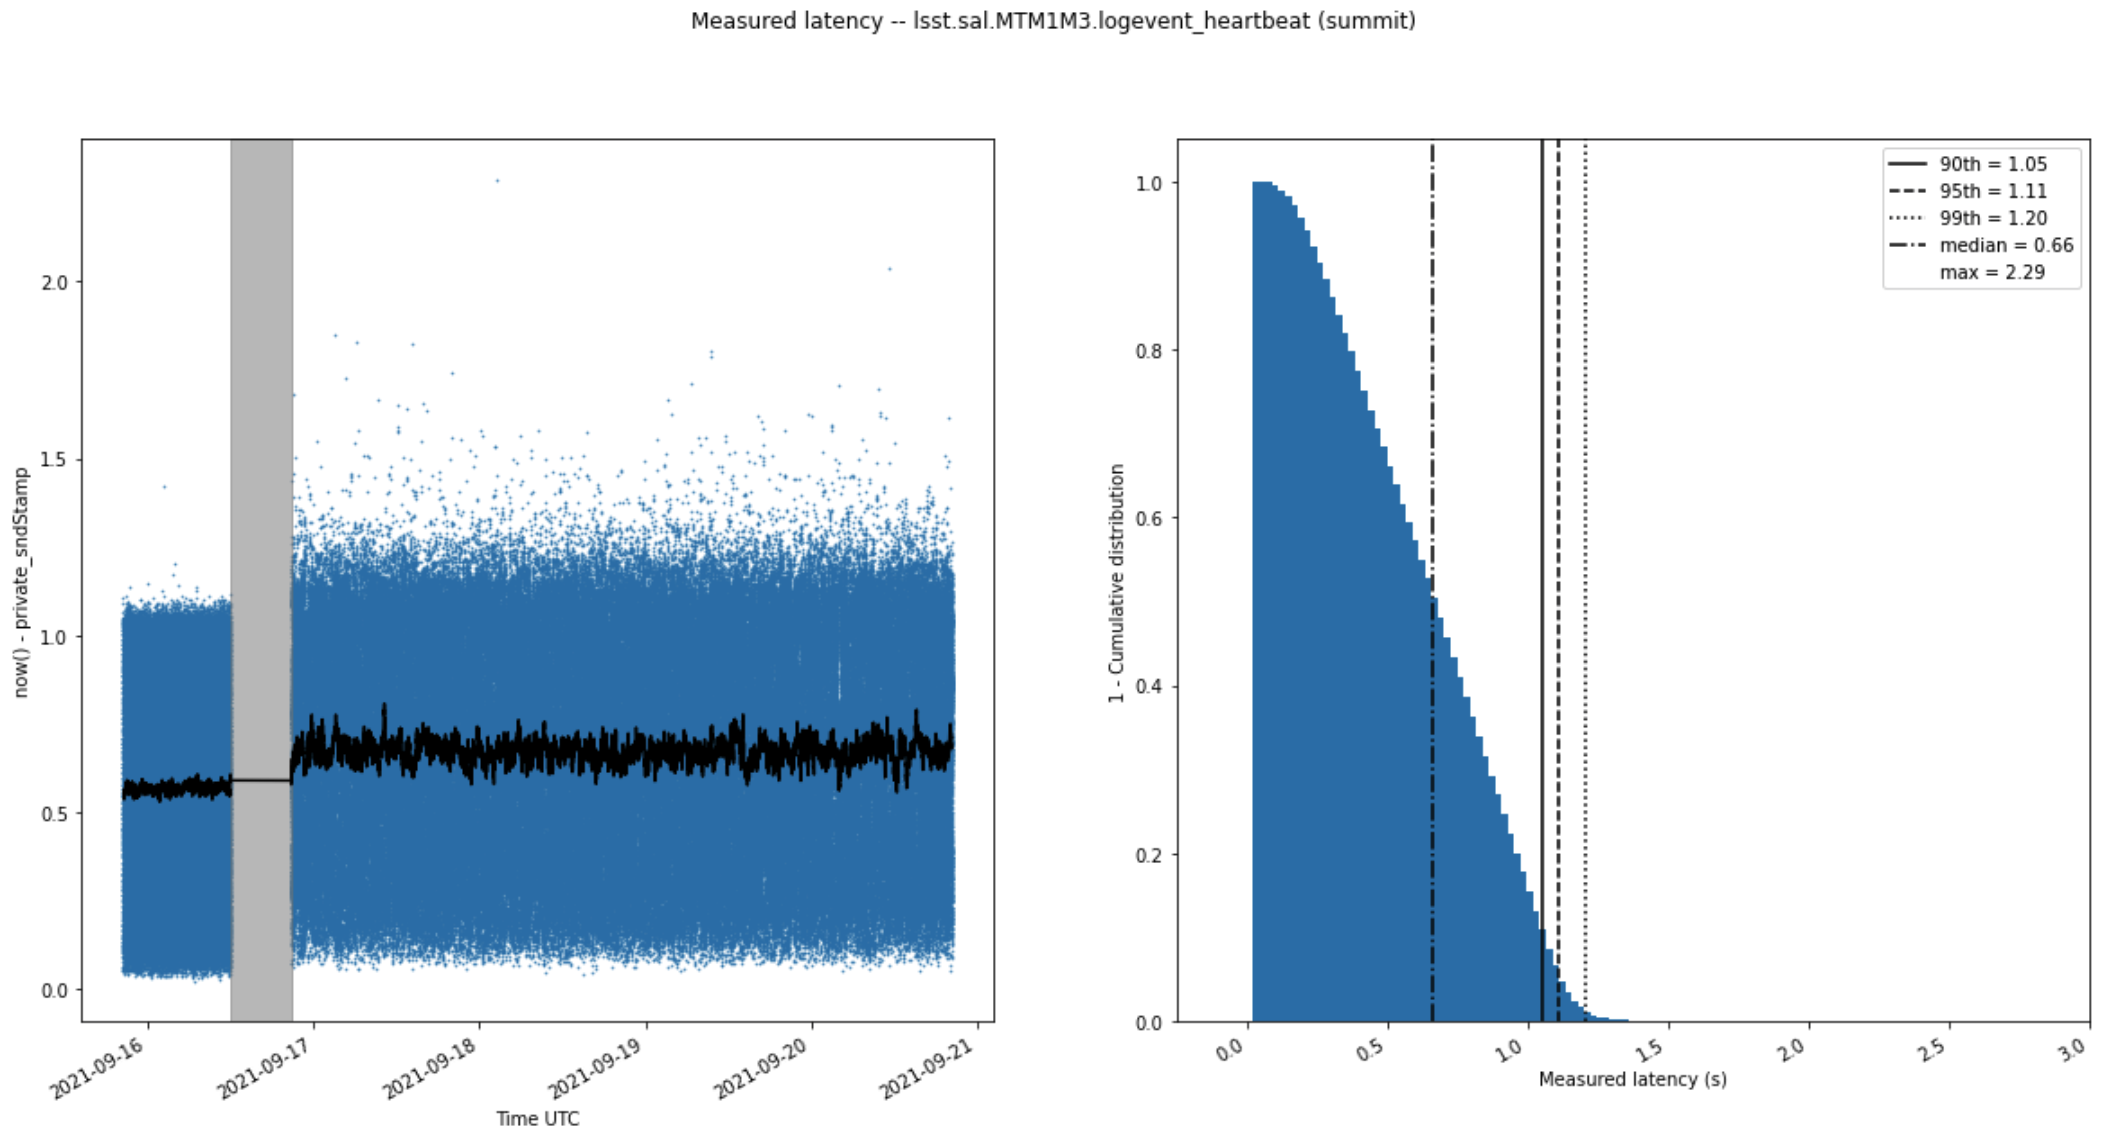
\includegraphics[width=4.03125in]{jira_imgs/1851.png}As with other plots
in this series, the left pane is the latency as a function of time and
the right is 1 minus the cumulative distribution. ~The lines show the
median, 90th, 95th and 99th percentiles. ~As can be seen in the plot,
the 99th percentile is 1.24 seconds which is significantly below the 4
seconds required from this test case. ~The maximum for this sample is
2.8 seconds. ~These easily satisfy the pass criteria for this test case.

}
\begin{tabular}{p{2cm}p{14cm}}
\toprule
Step 8 & Step Execution Status: \textbf{ Pass } \\ \hline
\end{tabular}
 Description \\
{\footnotesize
Document the procedure including latency distributions, time window, and
topics

}
\hdashrule[0.5ex]{\textwidth}{1pt}{3mm}
  Expected Result \\
{\footnotesize
\begin{itemize}
\tightlist
\item
  A document describing the process including the topic chosen and the
  time window.
\item
  The document shall be in the form on a notebook with saved outputs, or
  an instance of an nbreport.
\end{itemize}

}
\hdashrule[0.5ex]{\textwidth}{1pt}{3mm}
  Actual Result \\
{\footnotesize
See the attached notebook for implementation of the steps in this test.
~The script that generated the data file and the data file itself are
also attached.

}

\paragraph{ LVV-T2116 - Verify telemetry is uninterrupted for 5 days and can be analyzed via a
notebook at NCSA }\mbox{}\\

Version \textbf{1}.
Open  \href{https://jira.lsstcorp.org/secure/Tests.jspa#/testCase/LVV-T2116}{\textit{ LVV-T2116 } }
test case in Jira.

Test that telemetry is being recorded without missing messages for 5
days. ~This analysis is to be carried out using NCSA infrastructure.

\textbf{ Preconditions}:\\


Execution status: {\bf Pass }

Final comment:\\


Detailed steps results:

\begin{tabular}{p{2cm}p{14cm}}
\toprule
Step 1 & Step Execution Status: \textbf{ Pass } \\ \hline
\end{tabular}
 Description \\
{\footnotesize
Log in to whatever VPNs are necessary to access to the NCSA notebook
aspect of the RSP

}
\hdashrule[0.5ex]{\textwidth}{1pt}{3mm}
  Expected Result \\
{\footnotesize
VPN connection is active

}
\hdashrule[0.5ex]{\textwidth}{1pt}{3mm}
  Actual Result \\
{\footnotesize
Using the Cisco AnyConnect client, I have connected to the NCSA VPN
server. ~I authenticated with my NCSA Kerberos credentials answering the
2FA challenge using the DUO app on my phone.

}
\begin{tabular}{p{2cm}p{14cm}}
\toprule
Step 2 & Step Execution Status: \textbf{ Pass } \\ \hline
\end{tabular}
 Description \\
{\footnotesize
Log in to the NCSA notebook aspect:
https://lsst-lsp-stable.ncsa.illinois.edu/nb/\\
Make sure to choose a recent weekly and a large instance

}
\hdashrule[0.5ex]{\textwidth}{1pt}{3mm}
  Expected Result \\
{\footnotesize
The JupyterLab interface is displayed in the browser

}
\hdashrule[0.5ex]{\textwidth}{1pt}{3mm}
  Actual Result \\
{\footnotesize
After directing my browser to the appropriate URL,
https://lsst-lsp-stable.ncsa.illinois.edu/nb/, and logging in through
CILogon using my NCSA Kerberos credentials again and answering the 2FA
challenge using the DUO app on my phone, I now see the JupyterLab
environment in my browser window.\\[2\baselineskip]I chose the most
recent weekly: Weekly 2021\_37 (sciplat-lab:w\_2021\_37).

}
\begin{tabular}{p{2cm}p{14cm}}
\toprule
Step 3 & Step Execution Status: \textbf{ Pass } \\ \hline
\end{tabular}
 Description \\
{\footnotesize
Open a notebook:

\begin{enumerate}
\tightlist
\item
  Navigate to the File-\textgreater{}New-\textgreater{}Notebook
\item
  When prompted, select the LSST kernel
\end{enumerate}

}
\hdashrule[0.5ex]{\textwidth}{1pt}{3mm}
  Expected Result \\
{\footnotesize
An empty notebook running in the LSST kernel

}
\hdashrule[0.5ex]{\textwidth}{1pt}{3mm}
  Actual Result \\
{\footnotesize
Instead of going through the File menu, I went the route of using the
`+' button above the file browser. ~The result is the same. ~I currently
have a blank notebook running the LSST kernel as indicated in the upper
right. ~The notebook reports it is in the ``Idle'' state.

}
\begin{tabular}{p{2cm}p{14cm}}
\toprule
Step 4 & Step Execution Status: \textbf{ Pass } \\ \hline
\end{tabular}
 Description \\
{\footnotesize
Connect to the NCSA EFD\\
Note:The efd identifier is yet to be determined, but shall be ldf\_efd
or similar.

}
\hdashrule[0.5ex]{\textwidth}{1pt}{3mm}
  Example Code \\
{\footnotesize
from lsst\_efd\_client import EfdClient\\
efd = EfdClient('ldf\_efd')

}
\hdashrule[0.5ex]{\textwidth}{1pt}{3mm}
  Expected Result \\
{\footnotesize
A notebook with an instance of the `EfdClient` configured to talk to the
NCSA EFD

}
\hdashrule[0.5ex]{\textwidth}{1pt}{3mm}
  Actual Result \\
{\footnotesize
The actual string that I need to identify the appropriate EFD is
``ldf\_stable\_efd''. ~I was able to find this by using the
list\_efd\_names() method on the EfdClient class.\\[2\baselineskip]I now
have an efd client configured such that it is connected to the stable
version of the LDF EFD.

}
\begin{tabular}{p{2cm}p{14cm}}
\toprule
Step 5 & Step Execution Status: \textbf{ Pass } \\ \hline
\end{tabular}
 Description \\
{\footnotesize
Choose a topic to query and select a 5 day window of data. The window is
arbitrary, but must be explicit (not relative to now()) so that it can
be reproduced. Note that command topics shall be avoided for this
purpose since the semantics of private\_seqNum are different in the
context of commands than for other topic types

}
\hdashrule[0.5ex]{\textwidth}{1pt}{3mm}
  Expected Result \\
{\footnotesize
A time window and topic name that will be queried for the sequence
number

}
\hdashrule[0.5ex]{\textwidth}{1pt}{3mm}
  Actual Result \\
{\footnotesize
We choose the same topic name used in LVV-T2115. ~The topic is
``lsst.sal.MTM1M3.forceActuatorData''. ~For the time window, we take
advantage of the fact that the run was not exactly 5 days. ~We can show
that we have good message intake in a wider window than the strict 5
days by shifting for this test case so the window partially overlaps
that of LVV-T2115, but extends beyond the end probed there. ~the time
window starts one day later at 2021-05-26T00:00:00 and continues for 5
days following.\\[2\baselineskip]Because of technical difference in how
we interact with the database at NCSA vs at the summit, we use a
slightly different mechanism to query the database in this test case

}
\begin{tabular}{p{2cm}p{14cm}}
\toprule
Step 6 & Step Execution Status: \textbf{ Pass } \\ \hline
\end{tabular}
 Description \\
{\footnotesize
Care shall be taken to fix up the id column, private\_seqNum. It must be
monotonically increasing, but gets reset when the CSC is restarted. When
this happens an offset must be applied to the rest of the message ids in
order to produce a monotonically increasing sequence

}
\hdashrule[0.5ex]{\textwidth}{1pt}{3mm}
  Expected Result \\
{\footnotesize
A table-like object in memory with monotonically increasing message
numbers

}
\hdashrule[0.5ex]{\textwidth}{1pt}{3mm}
  Actual Result \\
{\footnotesize
We can tell the message numbers are monotonically increasing because the
difference between adjacent ids is never less than one.~ See cell 5 in
the attached notebook.

}
\begin{tabular}{p{2cm}p{14cm}}
\toprule
Step 7 & Step Execution Status: \textbf{ Pass } \\ \hline
\end{tabular}
 Description \\
{\footnotesize
Compute the difference between message ids via diff =
arr{[}`private\_seqNum'{]}{[}1:{]} - arr{[}`private\_seqNum'{]}{[}:-1{]}

}
\hdashrule[0.5ex]{\textwidth}{1pt}{3mm}
  Expected Result \\
{\footnotesize
A histogram normalized to the total number of samples from 1 to the
maximum number of the array diff.

}
\hdashrule[0.5ex]{\textwidth}{1pt}{3mm}
  Actual Result \\
{\footnotesize
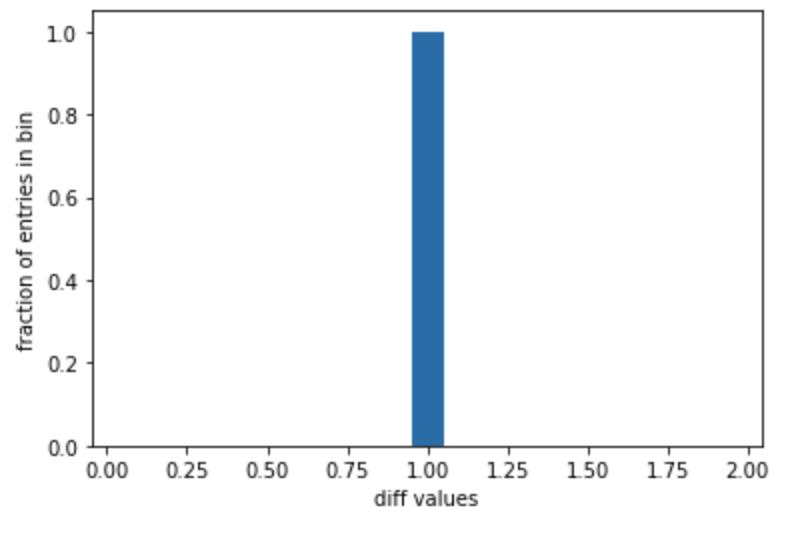
\includegraphics[width=3.12500in]{jira_imgs/1855.png}4The histogram does
indeed show that all elements end up in the bin containing the value 1.
Even more convincing is that when asking if all the elements in the
pairwise difference array are 1, the answer is ``yes'' (see cell
6).\\[3\baselineskip]

}
\begin{tabular}{p{2cm}p{14cm}}
\toprule
Step 8 & Step Execution Status: \textbf{ Pass } \\ \hline
\end{tabular}
 Description \\
{\footnotesize
Confirm that all values are one. Any larger numbers would indicate a gap
in messages

}
\hdashrule[0.5ex]{\textwidth}{1pt}{3mm}
  Expected Result \\
{\footnotesize
The result is that all differences in the histogram should be 1. Any
values larger than 1, which indicates a gap in messages, must be traced
to a problem with the CSC and not an issue with the EFD.

}
\hdashrule[0.5ex]{\textwidth}{1pt}{3mm}
  Actual Result \\
{\footnotesize
There were no gaps in the message IDs so no action was needed.

}
\begin{tabular}{p{2cm}p{14cm}}
\toprule
Step 9 & Step Execution Status: \textbf{ Pass } \\ \hline
\end{tabular}
 Description \\
{\footnotesize
Produce a report outlining this test

}
\hdashrule[0.5ex]{\textwidth}{1pt}{3mm}
  Expected Result \\
{\footnotesize
\begin{itemize}
\tightlist
\item
  A document describing the process including which topics/fields where
  used and what time window was selected.
\item
  The document shall be in the form of a notebook with saved outputs, or
  an instance of an nbreport
\end{itemize}

}
\hdashrule[0.5ex]{\textwidth}{1pt}{3mm}
  Actual Result \\
{\footnotesize
See the attached notebook

}

\paragraph{ LVV-T2115 - Verify telemetry is uninterrupted for 5 days and can be analyzed via a
notebook at the summit }\mbox{}\\

Version \textbf{1}.
Open  \href{https://jira.lsstcorp.org/secure/Tests.jspa#/testCase/LVV-T2115}{\textit{ LVV-T2115 } }
test case in Jira.

Test that telemetry is being recorded without missing messages for 5
days. ~This analysis is to be carried out using summit infrastructure.

\textbf{ Preconditions}:\\


Execution status: {\bf Pass }

Final comment:\\


Detailed steps results:

\begin{tabular}{p{2cm}p{14cm}}
\toprule
Step 1 & Step Execution Status: \textbf{ Pass } \\ \hline
\end{tabular}
 Description \\
{\footnotesize
Log in to whatever VPNs are necessary to access to the summit notebook
aspect of the RSP

}
\hdashrule[0.5ex]{\textwidth}{1pt}{3mm}
  Expected Result \\
{\footnotesize
VPN connection is active

}
\hdashrule[0.5ex]{\textwidth}{1pt}{3mm}
  Actual Result \\
{\footnotesize
I logged in to the summit VPN using the tunnelblick client with my
summit IPA credentials.~ The VPN is connected and active.

}
\begin{tabular}{p{2cm}p{14cm}}
\toprule
Step 2 & Step Execution Status: \textbf{ Pass } \\ \hline
\end{tabular}
 Description \\
{\footnotesize
Log in to the summit notebook aspect: https://summit-lsp.lsst.codes/nb\\
Make sure to choose a recent weekly and a large instance

}
\hdashrule[0.5ex]{\textwidth}{1pt}{3mm}
  Expected Result \\
{\footnotesize
The JupyterLab interface is displayed in the browser

}
\hdashrule[0.5ex]{\textwidth}{1pt}{3mm}
  Actual Result \\
{\footnotesize
I have opened the notebook aspect of the RSP by accessing the above URL
and using my GitHub credentials. ~I chose a large instance. ~The image
is ``Weekly 2021\_37 (SAL Cycle 0021, Build 005)''.

}
\begin{tabular}{p{2cm}p{14cm}}
\toprule
Step 3 & Step Execution Status: \textbf{ Pass } \\ \hline
\end{tabular}
 Description \\
{\footnotesize
Open a notebook:

\begin{enumerate}
\tightlist
\item
  Navigate to the File-\textgreater{}New-\textgreater{}Notebook
\item
  When prompted, select the LSST kernel
\end{enumerate}

}
\hdashrule[0.5ex]{\textwidth}{1pt}{3mm}
  Expected Result \\
{\footnotesize
An empty notebook running in the LSST kernel

}
\hdashrule[0.5ex]{\textwidth}{1pt}{3mm}
  Actual Result \\
{\footnotesize
JupyterLab is showing an empty notebook. ~The string in the upper right
says ``LSST''. ~The status in the lower left says ``Idle''.

}
\begin{tabular}{p{2cm}p{14cm}}
\toprule
Step 4 & Step Execution Status: \textbf{ Pass } \\ \hline
\end{tabular}
 Description \\
{\footnotesize
Connect to the summit EFD

}
\hdashrule[0.5ex]{\textwidth}{1pt}{3mm}
  Example Code \\
{\footnotesize
from lsst\_efd\_client import EfdClient\\
efd = EfdClient('summit\_efd')

}
\hdashrule[0.5ex]{\textwidth}{1pt}{3mm}
  Expected Result \\
{\footnotesize
A notebook with an instance of the `EfdClient` configured to talk to the
summit EFD

}
\hdashrule[0.5ex]{\textwidth}{1pt}{3mm}
  Actual Result \\
{\footnotesize
The example code executed without error and the notebook is once again
in the ``Idle'' phase.

}
\begin{tabular}{p{2cm}p{14cm}}
\toprule
Step 5 & Step Execution Status: \textbf{ Pass } \\ \hline
\end{tabular}
 Description \\
{\footnotesize
Choose a topic to query and select a 5 day window of data. The window is
arbitrary, but must be explicit (not relative to now()) so that it can
be reproduced. Note that command topics shall be avoided for this
purpose since the semantics of private\_seqNum are different in the
context of commands than for other topic types

}
\hdashrule[0.5ex]{\textwidth}{1pt}{3mm}
  Expected Result \\
{\footnotesize
A time window and topic name that will be queried for the sequence
number

}
\hdashrule[0.5ex]{\textwidth}{1pt}{3mm}
  Actual Result \\
{\footnotesize
We chose a high cadence topic because it should be the most likely to
uncover missing messages. ~The topic is
``lsst.sal.MTM1M3.forceActuatorData''. ~The time window was chosen to
overlap the time window used for other test cases in this test cycle for
consistency. ~The chosen time window is 2021-05-25T00:00:00Z + 5 days.

}
\begin{tabular}{p{2cm}p{14cm}}
\toprule
Step 6 & Step Execution Status: \textbf{ Pass } \\ \hline
\end{tabular}
 Description \\
{\footnotesize
Care shall be taken to fix up the id column, private\_seqNum. It must be
monotonically increasing, but gets reset when the CSC is restarted. When
this happens an offset must be applied to the rest of the message ids in
order to produce a monotonically increasing sequence

}
\hdashrule[0.5ex]{\textwidth}{1pt}{3mm}
  Expected Result \\
{\footnotesize
A table-like object in memory with monotonically increasing message
numbers

}
\hdashrule[0.5ex]{\textwidth}{1pt}{3mm}
  Actual Result \\
{\footnotesize
After correcting for the fact that the sequence resets to zero when a
CSC is restarted, we have a numpy array with monotonically increasing
values. ~See cell 6 for an indication of this. ~It should not print
anything if the sequence is monotonically increasing.

}
\begin{tabular}{p{2cm}p{14cm}}
\toprule
Step 7 & Step Execution Status: \textbf{ Pass } \\ \hline
\end{tabular}
 Description \\
{\footnotesize
Compute the difference between message ids via diff =
arr{[}`private\_seqNum'{]}{[}1:{]} - arr{[}`private\_seqNum'{]}{[}:-1{]}

}
\hdashrule[0.5ex]{\textwidth}{1pt}{3mm}
  Expected Result \\
{\footnotesize
A histogram normalized to the total number of samples from 1 to the
maximum number of the array diff.

}
\hdashrule[0.5ex]{\textwidth}{1pt}{3mm}
  Actual Result \\
{\footnotesize
Doing the above calculation results in an array where every entry is
one. ~See cell 10 for the mathematical evidence of this. ~I.e.
subtracting an array of all ones results in an array that sums to zero.
~We can also show that a histogram of the values has all elements in the
bin containing the value 1.\\
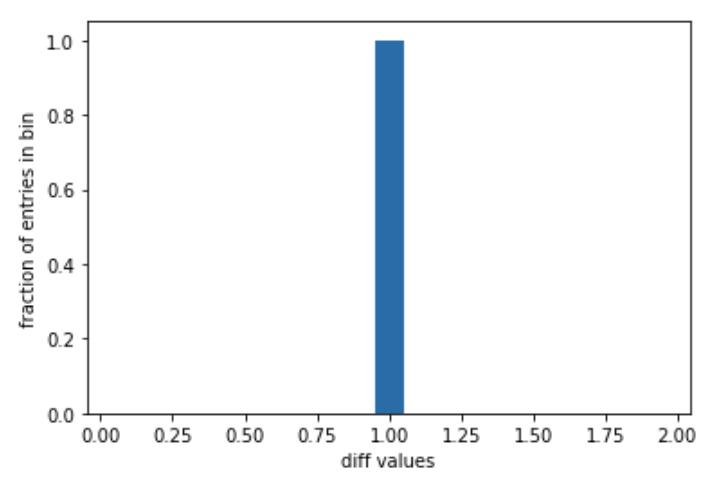
\includegraphics[width=3.12500in]{jira_imgs/1834.png}

}
\begin{tabular}{p{2cm}p{14cm}}
\toprule
Step 8 & Step Execution Status: \textbf{ Pass } \\ \hline
\end{tabular}
 Description \\
{\footnotesize
Confirm that all values are one. Any larger numbers would indicate a gap
in messages

}
\hdashrule[0.5ex]{\textwidth}{1pt}{3mm}
  Expected Result \\
{\footnotesize
The result is that all differences in the histogram should be 1. Any
values larger than 1, which indicates a gap in messages, must be traced
to a problem with the CSC and not an issue with the EFD.

}
\hdashrule[0.5ex]{\textwidth}{1pt}{3mm}
  Actual Result \\
{\footnotesize
There were zero instances in the 21373507 entries in our sample that
deviated from a value of one, so no further action was required.

}
\begin{tabular}{p{2cm}p{14cm}}
\toprule
Step 9 & Step Execution Status: \textbf{ Pass } \\ \hline
\end{tabular}
 Description \\
{\footnotesize
Produce a report outlining this test

}
\hdashrule[0.5ex]{\textwidth}{1pt}{3mm}
  Expected Result \\
{\footnotesize
\begin{itemize}
\tightlist
\item
  A document describing the process including which topics/fields where
  used and what time window was selected.
\item
  The document shall be in the form of a notebook with saved outputs, or
  an instance of an nbreport
\end{itemize}

}
\hdashrule[0.5ex]{\textwidth}{1pt}{3mm}
  Actual Result \\
{\footnotesize
See the attached rendered notebook for the report.

}




\newpage
\appendix
% Make sure lsst-texmf/bin/generateAcronyms.py is in your path
\section{Acronyms used in this document}\label{sec:acronyms}
\input{acronyms.tex}

\newpage

% generated from JIRA project LVV
% using template at /Users/krughoff/lsst_stack/conda/miniconda3-py38_4.9.2/envs/docsteady-env/lib/python3.7/site-packages/docsteady/templates/tpr-appendix.latex.jinja2.
% using docsteady version 2.2.3
% Please do not edit -- update information in Jira instead
\section{Traceability}

\begin{longtable}{p{3cm}p{3cm}L{9cm}}
\hline
\textbf{Test Case} & \textbf{VE Key} & \textbf{VE Summary} \\ \hline
\href{https://jira.lsstcorp.org/secure/Tests.jspa#/testCase/LVV-T2111}{LVV-T2111} &
 & \\ \hline
\href{https://jira.lsstcorp.org/secure/Tests.jspa#/testCase/LVV-T2112}{LVV-T2112} &
 & \\ \hline
\href{https://jira.lsstcorp.org/secure/Tests.jspa#/testCase/LVV-T2115}{LVV-T2115} &
 & \\ \hline
\href{https://jira.lsstcorp.org/secure/Tests.jspa#/testCase/LVV-T2116}{LVV-T2116} &
 & \\ \hline
\href{https://jira.lsstcorp.org/secure/Tests.jspa#/testCase/LVV-T2117}{LVV-T2117} &
 & \\ \hline
\end{longtable}


\end{document}
